% This is LLNCS.DEM the demonstration file of
% the LaTeX macro package from Springer-Verlag
% for Lecture Notes in Computer Science,
% version 2.4 for LaTeX2e as of 16. April 2010
%
\documentclass{llncs}
%
\usepackage{makeidx}  % allows for indexgeneration
%\usepackage[T2A]{fontenc} 
%\usepackage[utf8]{inputenc}
%\usepackage[english,russian]{babel}
\usepackage{graphicx}
\usepackage{indentfirst}
\usepackage{hyperref}
\usepackage{verbatim}
%
\begin{document}

\sloppy
%
%\frontmatter          % for the preliminaries
%
%\pagestyle{headings}  % switches on printing of running heads
%\addtocmark{Hamiltonian Mechanics} % additional mark in the TOC
%
%
%\tableofcontents
%
%\mainmatter              % start of the contributions
%
\title{From Abstract Parsing to Abstract Translation}
%
%\titlerunning{Hamiltonian Mechanics}  % abbreviated title (for running head)
%                                     also used for the TOC unless
%                                     \toctitle is used
%
\author{Semyon Grigorev\inst{1} 
\and Iakov Kirilenko\inst{2}
}
%
%\authorrunning{Ivar Ekeland et al.} % abbreviated author list (for running head)
%
%%%% list of authors for the TOC (use if author list has to be modified)
\tocauthor{Semyon Grigorev
, Iakov Kirilenko
}


\institute{St. Petersburg State University \\
198504, Universitetsky prospekt 28, Peterhof, St. Petersburg, Russia. \\
\email{rsdpisuy@gmail.com}
\and
St. Petersburg State University \\
198504, Universitetsky prospekt 28, Peterhof, St. Petersburg, Russia. \\
\email{jake@math.spbu.ru}
}

\maketitle              % typeset the title of the contribution

\begin{abstract}
String-embedded language transformation is one of the problems which can be faced during 
database and information system migration. The conventional solution which
is provided by a number of tools is based on run-time translation. We present a static 
\emph{abstract translation} approach which orignates from the \emph{abstract parsing} 
technique~\cite{AbstrParsing} initially developed for syntax analysis of string-embedded 
languages. We present abstract translation algorithm and some optimization techniques, and
discuss the results of its evaluation on a real-world industrial application.

%There are two approaches to 
%solve this problem: static translation or translation at run time. Our research deals 
%with the first one since solution for embedded language static translation problem do 
%not still exists. There is an abstract parsing algorithm~\cite{} for parsing of 
%string-embedded language. Parsing is close problem and in this article we propose abstract 
%parsing algorithm modification for application to string-embedded language translation. 
%We describe modifications of the basic algorithm which allow to translate embedded languages. 
%An algorithm of parsing forest minimization is also presented. We discuss some issues of 
%real-world dynamic SQL queries static translation and provide possible solutions. Finally, 
%we present results of implemented algorithm evaluation.

\keywords{Embedded languages, two-staged languages, string-embedded languages, abstract 
parsing,  abstract translation, LALR, dynamic SQL}
\end{abstract}

\section{Introduction}

Scalable high-performance graph analysis is an actual challenge.
There is a big number of ways to attack this challenge~\cite{Coimbra2021} and the first promising idea is to utilize general-purpose graphic processing units (GPGPU).
Such existing solutions, as CuSha~\cite{10.1145/2600212.2600227} and Gunrock~\cite{7967137} show that utilization of GPUs can improve the performance of graph analysis, moreover it is shown that solutions may be scaled to multi-GPU systems.
But low flexibility and high complexity of API are problems of these solutions.

The second promising thing which provides a user-friendly API for high-performance graph analysis algorithms creation is a GraphBLAS API~\cite{7761646} which provides linear algebra based building blocks to create graph analysis algorithms.
The idea of GraphBLAS is based on a well-known fact that linear algebra operations can be efficiently implemented on parallel hardware.
Along with that, a graph can be natively represented using matrices: adjacency matrix, incidence matrix, etc.
While reference CPU-based implementation of GraphBLAS, SuiteSparse:GraphBLAS~\cite{10.1145/3322125}, demonstrates good performance in real-world tasks, GPU-based implementation is challenging.

One of the challenges in this way is that real data are often sparse, thus underlying matrices and vectors are also sparse, and, as a result, classical dense data structures and respective algorithms are inefficient. 
So, it is necessary to use advanced data structures and procedures to implement sparse linear algebra, but the efficient implementation of them on GPU is hard due to the irregularity of workload and data access patterns.
Though such well-known libraries as cuSPARSE show that sparse linear algebra operations can be efficiently implemented for GPGPU, it is not so trivial to implement GraphBLAS on GPGPU. 
First of all, it requires \textit{generic} sparse linear algebra, thus it is impossible just to reuse existing libraries which are almost all specified for operations over floats.
The second problem is specific optimizations, such as masking fusion, which can not be natively implemented on top of existing kernels.
Nevertheless, there is a number of implementations of GraphBLAS on GPGPU, such as GraphBLAST~\cite{yang2019graphblast}, GBTL~\cite{7529957}, which show that GPGPUs utilization can improve the performance of GraphBLAS-based graph analysis solutions.
But these solutions are not portable because they are based on Nvidia Cuda stack.
Moreover, the scalability problem is not solved: all these solutions support only single-GPU, not multi-GPU computations.

To provide portable GPU implementation of GraphBLAS API we developed a \textit{SPLA} library\footnote{Source code available at: \url{https://github.com/JetBrains-Research/spla}}.
This library utilizes OpenCL for GPGPU computing to be portable across devices of different vendors.
Moreover, it is initially designed to utilize multiple GPGPUs to be scalable.
To sum up, the contribution of this work is the following.
\begin{itemize}
    \item Design of portable GPU GraphBLAS implementation proposed. The design involves the utilization of multiple GPUS. Additionally, the proposed design is aimed to simplify library tuning and wrappers for different high-level platforms and languages creation. 
    \item Subset of GraphBLAS API, including such operations as masking, matrix-matrix multiplication, matrix-matrix e-wise addition, is implemented. The current implementation is limited by COO and CSR matrix representation format and uses basic algorithms for some operations, but work in progress and more data formats will be supported and advanced algorithms will be implemented in the future.
    \item Preliminary evaluation on such algorithms as breadth-first search (BFS) and triangles counting (TC), and real-world graphs shows portability across different vendors and promising performance: for some problems Spla is comparable with GraphBLAST. Surprisingly, for some problems, the proposed solution on embedded Intel graphic card shows better performance than SuiteSparse:GraphBLAS on the respective CPU. At the same time, the evaluation shows that further optimization is required.
\end{itemize} 
\section{Graph-based Input Representation}
%\label{sec:RelatedWork}

As we mentioned above, the first stage of abstract parsing is static approximation
of relevant string values. Two main representations for approximated values were
used so far. In~\cite{StringExpr,ALVOR1,ALVOR2} the sets of potential string values 
are described using regular expressions; in~\cite{AbstrParsing} approximations are
represented in more implicit form as a solutions of a system of (recursive) dataflow 
equations. 

We did not find a way to scale either of these representations to abstract translation case. 
Instead, we represent the input stream for abstract translation via flow graph with one source and
one sink nodes and string-labeled edges. The labels of edges in this graph represent the results 
of constant propagation so that every path in input graph corresponds to one potential value of dynamic query. 
%Let we define that this path produce corresponded value and we will say that query contains lexical or syntax error if at least 
%one path which produce value with error exists in the corresponding graph. 
Moreover, we perform lexical analysis on graphs which converts the initial string-labeled graphs into
graphs, labeled by tokens.

% After that we define that input graph tokenization or lexical analysis is the process which convert input graph with string labels on edges (Fig.~\ref{pic1}) 
%to graph with tokens. The same way we define parsing or syntax analysis as the process which produce parsing forest by 
%input graph with edges labeled with tokens. As a result of parsing we have forest where each tree corresponds with query 
%value produced by any path in the input graph. When we describe abstract parsing and translation we assume that input 
%graph tokenization performed successfully.

Since any cycle in the input graph generates infinite sequence of tokens which upon translation is turned 
into infinite forest we simplify the graph even more. We replace each cycle with the single repetition. For example in the order to get regular approximation of query value set from code presented below we should build the next regular expression:
$$\text{"select * from "} \cdot (\text{\{tables.get(i)\}}|\varepsilon)^* \cdot \text{";"}$$
and the corresponding finite automaton (see Fig.~\ref{cyclesOrig}). Note that we do not care about approximation for \textit{tables.get(i)} expression because it depends on a constant propagation algorithm. But we will get the graph where cycle replaced with only one repetition of its body. The result of such approximation is presented in Fig.~\ref{cyclesApproximation}.

\begin{verbatim} 
query = "select * from ";
for(int i = 0; i < tables.size(); i++)
{
    if(i != 0) query += ", ";
    query += tables.get(i);
}
query += ";";
\end{verbatim}

\begin{figure}[t]
    \begin{center}
        \includegraphics[width=8cm,height=1.8cm]{graphs/cyclesOrig.eps}
        \caption{Correct finite automaton (graph representation)}
        \label{cyclesOrig}        
    \end{center}
\end{figure}



\begin{figure}[t]
    \begin{center}
        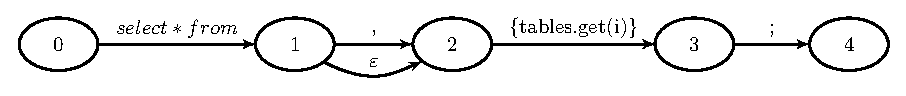
\includegraphics[width=8cm,height=0.8cm]{graphs/cyclesApproximation.eps}
        \caption{Result of cycles approximation}
        \label{cyclesApproximation}        
    \end{center}
\end{figure}


As you can see, in our example we do not produce strings like \verb|select * from tbl1, tbl2;| or \verb|select * from ;|. So, we can not check it. We process only two strings and all of them are in original infinite set: \verb|select * from tbl1;| and \verb|select * from, tbl1;|. As a result, we do not process all possible values but we process all variables used for query construction and it is enough for such tasks as code highlighting or transformations because all parts of expression are processed. 

Thus the graph becomes cycle-free and we can process all vertices in the topological order. While this drastic simplification is completely heuristic our experience of dynamic SQL translation for real information systems showed that DAG is still a good approximation for practical use.


%In the general case input graph can be arbitrary graph with cycles~\cite{AbstrParsing}. Cycles in the input graph may 
%be cause of infinite parsing. ut we have not found any practice implementations with problem of cycles processing fully 
%solved. We have found only two known implementations of abstract parsing: Alvor\footnote{Alvor is an Eclipse IDE plug-in 
%for statically checking of string-embedded SQL queries in Java programming language. This plug-in is based on LALR and GLR 
%abstract parsing and can be used either for incremental analysis or for offline checking of full code base. Alvor project 
%web site: \href{http://code.google.com/p/alvor/}{http://code.google.com/p/alvor/}} and the tool described in the Doh, Kim, 
%and Schmid's article. Alvor use stack size limitation to avoid infinite processing of cycles. Doh, Kim, and Schmid's 
%implementation of LALR(1)-based abstract parsing cannot be found and article does not contain practice solution of 
%cycles processing problem. In sum, efficient arbitrary graph with cycles processing in abstract parsing is an open question.
	

%For practical usage it is very important that information systems can contain a big 
%number of dynamic queries and each one of them can contains hundreds of 
%branches~\cite{TiunovaUIInt}. The necessity of analyzing all possible values for 
%each query can cause  performance problems and exponential growth of required 
%resources.

As an example consider the following code snippet:

\begin{verbatim} 
   (1) IF @X = @Y
   (2) SET @TABLE = '#tbl1'
   (3) ELSE
   (4) SET @TABLE = 'tbl2'
   (5) SET @S = 'SELECT x FROM ' + @TABLE
   (6) EXECUTE (@S)
\end{verbatim}

Variable \verb @S \ contains dynamically generated query and can have two potential values at the point of query execution. 
During approximation we can build a graph which represents the set of potential values of the variable \verb @S \ at the 
line 6. Each edge of this graph is labeled by a token which represents a part of the query (see Fig.~\ref{pic1}).

\begin{figure}
    \begin{center}
        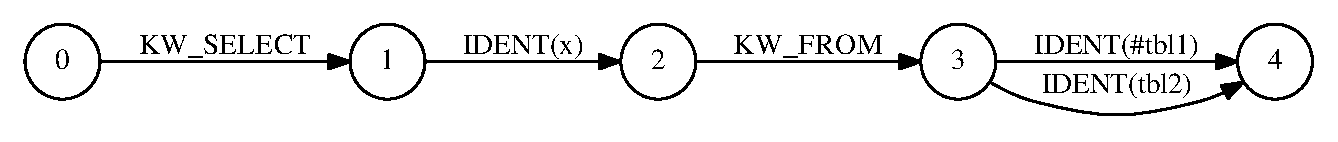
\includegraphics[width=8cm,height=0.8cm]{graphs/simple_sql.eps}
        \caption{Tokenized input graph}
        \label{pic1}        
    \end{center}
\end{figure}

Note that real-world systems can communicate with other systems source of which may be inaccessible to analyze. These systems can contain parts of queries to process and we should use some approximations. For example, clients applications of information system can sent conditions for filters (conditions for \verb|where| clause of \verb|select| statement) as part of requests.





\section{Abstract translation}
\label{sec:AbstractTranslation}

To solve a problem of dynamic queries translation we should calculate new values for all variables used 
for queries construction. If we want to create static translator then result of translation should not 
require any changes after translation is finished. Basic idea is that we should try to apply classical 
translation techniques to each possible value of dynamic query. So we should build parsing forest and 
translate each of trees, and calculate new string values based on translation result.

Semantic equivalent constructions of source and target languages should have similar syntax in order to 
abstract translation could be applied. If this constraint is not satisfied then solution could not be
 reduced to new values calculation for existing variables. New variable creation may be required and 
this fact can significantly increase complexity of solution and corresponded analysis.

Also we suppose that input data structure for parser is direct acyclic graph (DAG) with one source and 
one sink vertices. Our experience of dynamic SQL translation for real information system shows that DAG 
is a good approximation of the dynamically constructed expressions set for practical use. We should replace 
all cycles with single repetition during approximation to get such graph. This way we can process all vertices 
in the topological order and avoid the problem with cycles processing previously discussed.

We propose to modify basic LALR-based algorithm of abstract parsing to solve the problem of abstract 
translation. The original parsing algorithm targeted to recognition, not translation, and it does not 
support semantics calculation. This fact allows to operate only with tokens type, not tokens values. 
It is possible to merge states like in GLR-algorithm\footnote{Generalized Left-to-right Rightmost 
derivation -- LR-based parsing algorithm for arbitrary (ambiguous) context-free grammars 
processing~\cite{Grune}.}. This way we can avoid problems with size of states set and parsing result.
 If we want to translate input expression to another language then we should keep all information 
about tokens values. 

One of the possible solution of translation is abstract parsing algorithm with mechanism of stack 
splitting for semantic calculation support. It disallow to merge states and we should create new 
copies of stack on each branch in input graph and get exponential memory usage in worst case. 
Note that there is a big number of dynamic expressions which require exponential resources to 
analyze in the real world information systems. 

For example parser states for vertex $V_3$ in picture~\ref{pic4} should be equal for 2 input edges
but if we want to calculate semantics, then we get two different states because identifiers has 
different values.

\begin{figure}
    \begin{center}
        \includegraphics[width=11cm,height=1.4cm]{graphs/states_example.eps}
        \caption{Graph with states possible to merge.}
        \label{pic4}
    \end{center}
\end{figure}

Queries which contains a huge number of branches is a big problem. The number of states is an 
exponential function of the Nnumber of branches because for each branch we should produce $n*k$ 
states where $n$ is a number of states in root of fork vertex and $k$ is a number of branches. 
One of the most frequent example of queries with big number of branches is \verb|select| query. 
Each of fields to select can be calculated with if-statement or case-statement. Example of such 
graph presented in picture~\ref{pic5}.

\begin{figure}
    \begin{center}
        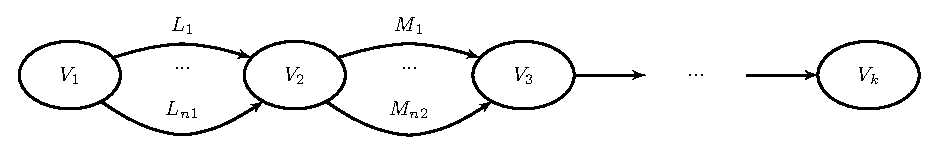
\includegraphics[width=11cm,height=2cm]{graphs/big_res.eps}
        \caption{Graph which require an exponential resources for translation.}
        \label{pic5}
    \end{center}
\end{figure}

If we use only sequentially concatenated if-statements then the number of parsing trees is $2^n$ 
where $n$ is a number of if-statements (or number of branches). In the real-world systems we 
have faced the queries which contains more than 100 branches. Full forest calculation by naive 
adaptation of abstract parsing is impossible for such queries. The set of states to be processed
 minimization is an actual problem for real-world systems.

\subsection{Optimization of the abstract translation algorithm}
\label{sec:Optimizations}

We propose the following solution of forest size minimization problem. We have previously discussed 
that the result of translation is new values for all variables which were used for queries construction. 
It is sufficient to construct not the full forest but only the minimal set of trees such that after 
translation every variable gets new value.This way, we can process not all paths in the input graph 
but only minimal set which contains all edges. Note that we cannot calculate this set before parsing 
because we cannot be sure that every path produces syntax correct values. If some path contains 
error than the tree is not constructed and we lose information about variables. For example let
we try to process the graph presented in picture~\ref{pic6}.

\begin{figure}
    \begin{center}
        \includegraphics[width=11cm,height=2cm]{graphs/paths.eps}
        \caption{Graph for minimal paths set selection.}
        \label{pic6}
    \end{center}
\end{figure}

One possible set of paths which we can be calculated before syntax analysis is $\{(L_1; M_1); (L_2; M_2)\}$. 
But every path contains syntax errors and the result forest is empty instead of containing 2 trees. 
We should choose another set (for example $\{(L_1; M_2); (L_2; M_1)\}$) to get correct result. So, 
path calculation is iterative process. We should perform states filtering during syntax analysis 
for each vertex with multiple input edges. Let we describe steps of the process.

\begin{itemize}
    \item \textbf{Initial state.} Set of states for vertex is empty. 
    \item \textbf{Step.} For each step if the current vertex has multiple input edges then we should add new state to states set for current vertex if any of the next conditions is true.
    \begin{itemize}
        \item New state corresponds with path which contains edges which are not contained in any of paths corresponded with states in the currently processed set. 
        \item New state corresponds with parser state which is not presented in the currently processed set.
    \end{itemize}

\end{itemize}

Described algorithm pseudo code is presented below.
\begin{verbatim}
/*
V – list of input graph vertices in the topological order.
v_s – start vertex of input graph.
*/

let filterStates v =
    let groupedByParserState =
        v.States.GroupBy (fun state -> state.Item)

    v.States = Set.empty

    for group in groupedByParserState do
        /* Each state corresponds with path from v_s to v.
         Set of paths specify set of edges of graph E_s.
         We should construct minimal set of paths which
         contains all edges of E_s. The next greedy algorithm
         can be applied to solve this problem.
         1) Order paths by length ascent.
         2) While current path contains edges not in
         the result set add this path in the result set.*/
        let ordered = 
            group.OrderBy (fun s -> -1 * s.Path.Lenght)
        for s in ordered do
            if (s.Path contains edges which 
                not in any path from result set) 
            then v.States.Add s

for v in V do
    v.States <- … /*step of syntax analysis*/
    /*If input degree of the vertex v more 
      then 1 then try to filter states.*/
    if v.InEdges.Count > 1 then filterStates v

\end{verbatim}

This way we can get states set which contains all parser states from input set but is not greater 
than it. Corresponded paths contains all possible edges in processed subgraph. Described algorithm
of filtration allows to increase performance of parsing by decreasing a number of parsing trees.

\section{Evaluation}

This section describes the methodology and answers the following research questions.

\begin{enumerate}
    \item Does fusion via distillation give any benefits at the software and hardware levels?
    \item What are the properties of the generated hardware?
    \item Does the generated hardware outperform software implementations?
\end{enumerate}

\subsection{Methodology}

Our focus is on creating a basis for future research and experiments, thus we make our experiments as much reproducible as possible\footnote{\url{https://github.com/sedwards-lab/fhw/tree/sparse-linear-algebra-distillation/examples/QTreeBenchmarks/diploma/verilog-bool-no-nnz-inlined} (online; accessed:
2022-06-07) Here one could find all the results. For each benchmark all statistics are specified: matrix names, their sizes, collected metrics for both hardware and software benchmarks.}. We benchmarked the following list of chained functions. The choice is prompted by the current state of the distiller: at the moment, it does not successfully distill matrix multiplication. However, the functions are still practical enough, for example, chained addition could be seen in Luby's maximal independent set algorithm and clearly describe the applicability of the proposed approach.

\begin{itemize}
    \item \mintinline{Haskell}{mAdd (==False) (||) (mAdd (==False) (||) m1 m2) m3}
    \item \mintinline{Haskell}{mask (mAdd (== False) (||) m2 m3) (m1)}
    \item \mintinline{Haskell}{map (==Zero) (to_nat) (mAdd (==False) (||) m1 m2}
    \item \mintinline{Haskell}{map (==Zero) (to_nat) (kron (==False) (&&) m1 m2}
\end{itemize}

Above, \mintinline{Haskell}{Zero} and \texttt{to\_nat} are corresponding definitions for Peano arithmetics, since the \texttt{.pot} language does not have any primitives. For the same reason, we operated with boolean matrices. Such functions could be abstracted with free variables and then instantiated in the emitted Haskell code. However, to get maximum from distillation, we provided all the information about the functions. 

For these functions, we compared the execution time of distilled and not distilled hardware generated circuits, execution time of original and distilled Haskell code and reference \textit{Suite Sparse}\footnote{\url{https://github.com/DrTimothyAldenDavis/GraphBLAS} (online; accessed:
2022-06-07), Suite Sparse library sources.}\textsuperscript{,}\footnote{The library also uses different variations of coordinate formats (opaque to the user) and not a quadtree representation.} variants of these functions in C\texttt{++}. Note that SuiteSparse does not support recursive data types, thus only the first two function chains were implemented in SuiteSparse (since Peano number is essentially a linked list). We did not replace Peano numbers with integers, so our experiments could be interpreted easier. For hardware experiments we collected execution time and the number of memory writes and reads, to access how well fusion is performed. For software experiments we only measured the execution time. Also note that we measured only the time, required to execute the lines above, not including any IO, required to get and evaluate function arguments. But in hardware benchmarks we measured the time required to pass arguments into the circuit's memory, because such IO is inevitable. It is tricky to make such measures in Haskell due to laziness, thus the programs were compiled with \texttt{--fno-full-laziness} to turn off memoization. Also all the arguments were forced to normal form via \texttt{force} and \texttt{evaluate}. Haskell programs were compiled\footnote{GHC 8.10.4.} with \texttt{-O2 --fno-full-laziness} and Suite Sparse was compiled with default flags and linked as a shared library to C\texttt{++} code.

We took matrices from SuiteSparse matrix collection with sizes ranging from \texttt{64x64} to \texttt{512x512}. We limited ourselves with such sizes due to the fact that this is the maximum sizes that fit into \texttt{bram} with $2^{16}$ address space. Such number of \texttt{bram} blocks is available only on really expensive FPGA boards, thus in practice sizes would be smaller to achieve better utilization. Once again, it models the situation when data fits into the cache, since \texttt{bram} in our circuits will operate as a cache in real application.

\subsection{Experiments}

Table~\ref{tab:bench_results} shows the results of all execution time benchmarks. To evaluate execution time for hardware simulation, implementation stage was performed to assess the maximum frequency of FPGA device used for synthesis and implementation, and the number of execution cycles was multiplied by the number of nanoseconds a clock cycle takes. The frequencies were equal within the same benchamark set, i.e., frequency was not affected by distillation. We used \texttt{xcu250figd2104-2L} device\footnote{\url{https://www.xilinx.com/products/boards-and-kits/alveo/u250.html}  (online; accessed:
2022-06-07)} for synthesis and implementation stages. It is not really a casual and affordable chip, but it contains enough \texttt{bram} for our evaluation to see scalability. In the table a median across several benchmarks is shown. 

As it could be seen, distillation steadily increases performance: up to 2x speedup for hardware simulation and up to 3x for software benchmarks. The results are maintained within the borders of the corresponding confidence interval and the borders are not shown for brevity. Hardware speedup is lower due to the different execution semantics, dataflow is not reduction-based and distillation is a reduction-based transformation. Note that generated hardware appears to be less performant than both Haskell and C\texttt{++}, which a bit contradicts the results from~\cite{oldfhw}. For hardware benchmarks \texttt{time (IO)} shows the execution time including the time needed to transfer the data though the arguments, \texttt{time (no IO)} does not include it in its turn. It could be seen that not all the benchmarks are computationally extensive enough to cover memory transferring costs, but for more complex examples the ratio would be better. Since we basically transfer the matrices node by node from a file in the testbench, we have probably the lowest possible latency, and in practice it would be higher if reading from DDR, however the bandwidth could be increased. Noticeably, running times for \texttt{mMaskAdd} for C\texttt{++} and distilled Haskell are similar, which shows that fusion really provides some extra performance: SuiteSparse at the moment does not implement any fusion.

Table~\ref{tab:mem_results} summarizes the ratios between distilled and not distilled hardware circuits memory reads and writes. Since in general case distillation removes extra pattern matching, essentially it saves memory reads and writes. The eventual number of memory reads and writes is implementation dependent, thus the table shows what share of speedup is prompted by saving memory operations. Distillation successfully reduces the number of memory accesses, about 15\% on average. \texttt{mMapKron} has a bit higher ratio due to the fact that \texttt{Nat} numbers require additional memory accesses, since the type is recursive. It could also be seen that a major part of speedups is attributed to saved memory accesses. 

Finally, table~\ref{tab:resource_util} shows device resources utilization ratios between distilled and not distilled hardware circuits and frequencies. Columns are device primitives: registers, lookup tables, \texttt{bram} blocks or multiplexers. Utilization for both types of circuits is below 1\% of available resources on the device, except for the memory. Memory blocks utilization is about 30\% (since we choose larger \texttt{brams} to store larger matrices). Apart from that, distilled circuits could have both higher and lower utilization. Since the hardware generation is primarily syntax-directed it follows from the distilled program structure. For example, distillation might glue two recursive functions into one (in that case, memory utilization would be lower, because each cluster of mutually recursive functions possesses its own heap) or make more recursive functions than in the original program. The frequencies are the same, however, they possibly could be made better with more intelligent buffer allocation.

\subsection{Discussion}
Answering the research questions above.

\begin{enumerate}
    \item Fusion gives significant benefits, however at the hardware level the benefits are a bit smaller since hardware semantics is not reduction based. The benefits at the hardware level are mostly determined by the reduced number of memory accesses (each access takes 2 clock cycles). Notably, distilled Haskell implementation of \texttt{mMaskAdd} has similar performance with C\texttt{++}. 
    \item Device utilization is low, but such circuits could be copied on the same device to provide better utilization and higher parallelism. Resource utilization might be both better and worse after distillation, depending on the transformed program itself since translation is syntax-directed. Frequency could be increased by more intelligent buffering strategy.
    \item Although we use low-latency design with \texttt{bram}s that take 2 clock cycles per request and transfer matrices from files, which does not have any latency in simulation, we get slower execution time than Haskell and C\texttt{++} counterparts. It could be partly due to excessive buffering performed by FHW at the moment. Also there is no pipelining for recursive calls, i.e. only one set
of function argument tokens are allowed to enter a tail-recursive function call until a result is finally generated. Further CPS transformation hinders parallelization, which could be made more explicit with SSA. Some other optimizations exist that may significantly influence the performance. Also, since device utilization is about 1\%, such circuits could be copied on one device and provide more parallelism. A more detailed discussion could be found at~\cite{Edwards2019FHWP}.
\end{enumerate}

Distillation clearly showed its applicability to optimization of sparse linear algebra routines and notably it still could be combined with other techniques, like rewrite rules to achieve better results. High-level synthesis has a room for improvements by increasing pipelining, parallelism and frequency and the generated hardware could be improved from usability perspective: a support for arbitrary sized matrices is desirable. Thus we will focus on these directions. Probably a better solution would be to embed \texttt{.pot} language into e.g. Haskell to leverage its type system (to be able to use some rewrite rules as well), and add support for primitive types and parallel primitives to be able to conduct a more scalable comparison with SuiteSparse (since SuiteSparse is multithreaded). For such embedding different execution models could be implemented, including hardware synthesis, for which SSA form of GRIN looks promising, as well as extra optimizations shipped with GRIN. For hardware synthesis, an interesting direction is achieving predictable results in hardware from certain modifications in software. This property partly holds for the current approach, since the translation is syntax- directed. More information on this could be found at~\cite{predict}.

\pagebreak

\begin{table}[t]
\scriptsize
\centering
\caption*{mAddAdd}
\begin{tabular}{|c|c|c|c|c|c|c|c|c|c|} 
\hline
\rowcolor{LightBlue}
\multicolumn{3}{|c|}{Matrices dimensions} & Haskell & Haskell (distilled) & \multicolumn{2}{c|}{FHW} & \multicolumn{2}{c|}{FHW (distilled)} & {C\texttt{++}}\\
% \rowcolor{LightBlue}
\hline
m1 & m2 & m3 & time & time & time (no IO) & time (IO) & time (no IO) & time (IO) & time \\ 
\hline
64 & 64 & 64 & 29 us & 20 us & 76 us & 170 us & 64 us & 158 us & 14 us\\ 
128 & 128 & 128 & 94 & 79 & 146 & 476 & 134 & 469 & 30 \\
256 & 256 & 256 & 123 & 103 & 202 &  681 & 168 & 662 & 44\\
512 & 512 & 512 & 219 & 143 & 474 & 1192 & 375 & 1093 & 49\\
\hline
\end{tabular}

\caption*{mMaskAdd}
\begin{tabular}{|c|c|c|c|c|c|c|c|c|c|} 
\hline
\rowcolor{LightBlue}
\multicolumn{3}{|c|}{Matrices dimensions} & Haskell & Haskell (distilled) & \multicolumn{2}{c|}{FHW} & \multicolumn{2}{c|}{FHW (distilled)} & {C\texttt{++}}\\
% \rowcolor{LightBlue}
\hline
m1 & m2 & m3 & time & time & time (no IO) & time (IO) & time (no IO) & time (IO) & time \\ 
\hline
64 & 64 & 64 & 10 us & 7 us & 64 us & 133 us & 46 us & 111 us & 18 us\\ 
128 & 128 & 128 & 38 & 30 & 118 & 322 & 75 & 292 & 33 \\
256 & 256 & 256 & 48 & 42 & 168 &  498 & 104 & 456 & 46\\
512 & 512 & 512 & 126 & 76 & 400 & 762 & 300 & 729 & 65\\
\hline
\end{tabular}

\caption*{mMapAdd}
\begin{tabular}{|c|c|c|c|c|c|c|c|c|c|} 
\hline
\rowcolor{LightBlue}
\multicolumn{3}{|c|}{Matrices dimensions} & Haskell & Haskell (distilled) & \multicolumn{2}{c|}{FHW} & \multicolumn{2}{c|}{FHW (distilled)} & {C\texttt{++}}\\
% \rowcolor{LightBlue}
\hline
m1 & m2 & m3 & time & time & time (no IO) & time (IO) & time (no IO) & time (IO) & time \\ 
\hline
64 & 64 & --- & 45 us & 37 us & 189 us & 253 us & 137 us & 202 us & ---\\ 
128 & 128 & --- & 162 & 105 & 524 & 685 & 397 & 579 & --- \\
256 & 256 & --- & 312 & 216 & 1047 &  1360 & 680 & 986 & ---\\
512 & 512 & --- & 436 & 273 & 1346 & 1776 & 900 & 1330 & ---\\
\hline
\end{tabular}

\caption*{mMapKron}
\begin{tabular}{|c|c|c|c|c|c|c|c|c|c|} 
\hline
\rowcolor{LightBlue}
\multicolumn{3}{|c|}{Matrices dimensions} & Haskell & Haskell (distilled) & \multicolumn{2}{c|}{FHW} & \multicolumn{2}{c|}{FHW (distilled)} & {C\texttt{++}}\\
% \rowcolor{LightBlue}
\hline
m1 & m2 & m3 & time & time & time (no IO) & time (IO) & time (no IO) & time (IO) & time \\ 
\hline
2 & 64 & --- & 64 us & 36 us & 212 us & 242 us & 94 us & 125 us & ---\\ 
2 & 128 & --- & 137 & 68 & 434 & 502 & 199 & 266 & --- \\
2 & 256 & --- & 364 & 126 & 1004 &  1188 & 449 & 636 & ---\\
4 & 128 & --- & 302 & 94 & 694 & 763 & 330 & 401 & ---\\
\hline
\end{tabular}



\caption{Execution time}
\label{tab:bench_results}

\end{table}
\begin{table}[h]
\scriptsize
\begin{minipage}{0.45\linewidth}
\centering
\caption*{mAddAdd}
\begin{tabular}{|c|c|c|c|c|c|c|} 
\hline
\rowcolor{LightBlue}
\multicolumn{3}{|c|}{Matrices dimensions} & \multicolumn{2}{c|}{Ratio ($\frac{FHW}{FHW_{distilled}}$)}\\
% \rowcolor{LightBlue}
\hline
m1 & m2 & m3 & writes & reads\\ 
\hline
64 & 64 & 64 & 1.10 & 1.15\\ 
128 & 128 & 128 & 1.02 & 1.05\\
256 & 256 & 256 & 1.03 & 1.06\\
512 & 512 & 512 & 1.10 & 1.16\\
\hline
\end{tabular}
\end{minipage}
\begin{minipage}{0.45\linewidth}
\centering
\caption*{mMaskAdd}
\begin{tabular}{|c|c|c|c|c|c|c|} 
\hline
\rowcolor{LightBlue}
\multicolumn{3}{|c|}{Matrices dimensions} & \multicolumn{2}{c|}{Ratio ($\frac{FHW}{FHW_{distilled}}$)}\\
% \rowcolor{LightBlue}
\hline
m1 & m2 & m3 & writes & reads\\ 
\hline
64 & 64 & 64 & 1.13 & 1.26\\ 
128 & 128 & 128 & 1.06 & 1.11\\
256 & 256 & 256 & 1.08 & 1.09\\
512 & 512 & 512 & 1.10 & 1.16\\
\hline
\end{tabular}
\end{minipage}
\begin{minipage}{0.45\linewidth}
\centering
\caption*{mMapAdd}
\begin{tabular}{|c|c|c|c|c|c|c|} 
\hline
\rowcolor{LightBlue}
\multicolumn{3}{|c|}{Matrices dimensions} & \multicolumn{2}{c|}{Ratio ($\frac{FHW}{FHW_{distilled}}$)}\\
% \rowcolor{LightBlue}
\hline
m1 & m2 & m3 & writes & reads\\ 
\hline
64 & 64 & --- & 1.10 & 1.21\\ 
128 & 128 & --- & 1.07 & 1.14\\
256 & 256 & --- & 1.07 & 1.19\\
512 & 512 & --- & 1.10 & 1.21\\
\hline
\end{tabular}
\end{minipage}
\hfill
\begin{minipage}{0.45\linewidth}
\centering
\caption*{mMapKron}
\begin{tabular}{|c|c|c|c|c|c|c|} 
\hline
\rowcolor{LightBlue}
\multicolumn{3}{|c|}{Matrices dimensions} & \multicolumn{2}{c|}{Ratio ($\frac{FHW}{FHW_{distilled}}$)}\\
% \rowcolor{LightBlue}
\hline
m1 & m2 & m3 & writes & reads\\ 
\hline
2 & 64 & --- & 1.71 & 1.88\\ 
2 & 128 & --- & 1.72 & 1.87\\
2 & 256 & --- & 1.65 & 1.83\\
4 & 128 & --- & 1.81 & 1.91\\
\hline
\end{tabular}
\end{minipage}

\caption{Memory accesses}
\label{tab:mem_results}
\end{table}

\begin{table}[h]
\scriptsize
\centering
\begin{tabular}{|l|c|c|c|c|c|c|c|c|c|} 
\hline
\rowcolor{LightBlue}

{Benchmark} & \multicolumn{8}{c|}{Ratio (${\frac{FHW}{FHW_{distilled}}}$)} & {Frequency}\\
\hline
{} & FDRE & LUT3 & LUT6 & LUT5 & LUT4 & LUT2 & RAMB36E2 & MUXF7 & {} \\
% \rowcolor{LightBlue}
\hline
mAddAdd & 0.3 & 0.3 & 0.3 & 0.5 & 0.3 & 0.3 & 0.5 & 0.5 & 200 MHz\\ 
mMaskAdd & 0.5 & 0.5 & 0.7 & 0.4 & 0.7 & 0.5 & 0.7 & 0.6 & 200 MHz\\
mMapAdd & 1 & 0.9 & 0.9 & 1.2 & 1 & 1.1 & 1.1 & 1.2 & 200 MHz\\
mMapKron & 1.5 & 1.5 & 1.3 & 2 & 2 & 1.8 & 1.4 & 1.7 & 200 MHz\\
\hline
\end{tabular}
\caption{Resource utilization}
\label{tab:resource_util}
\end{table}
\pagebreak

\section{Conclusion and Future Work}

We present !!!

Our evaluation shows that !!!

First direction for future research is a more detailed CFPQ algorithms investigation.
We should do More evaluation on sparse matrices on GPGPUs.

Also it is nesessary to implement and evaluate solutions for graphs which is not fit in RAM.
There is a set of technics for huge matrices multiplication.
Is it possible to dopt it for CFPQ

Another direcion is a dataset improvement.
More data.
More grammars/queries.


%
% ---- Bibliography ----
%
\begin{thebibliography}{}
  
\bibitem{RelaxedLALR}
Ефимов А.А., Кириленко Я.А. Построение ослабленного LALR-транслятора на основе анализа грамматики на избыточность // Системное программирование. Т. 4, вып. 1, 2009. С. 79–103.  

\bibitem{mart}
Мартыненко Б.К. Языки и трансляции. Издательство Санкт-Петербургского университета, 2008. 257 с. 

\bibitem{TiunovaUIInt}
Мосиенко М.А., Тиунова А.Е. Интеграция программной логики с пользовательским интерфейсом при реинжиниринге приложений // Системное программирование. Т. 1, вып. 1, 2004. С. 199–224.

\bibitem{NetDbTransform}
Трошин С.Л. Преобразование сетевых баз данных в реляционные: задачи и подходы // Системное программирование. Т. 1, вып. 1. 2004. С. 282–310.

\bibitem{OpenSystemsDBMS}
Shapot M., Popov E. Database reengineeing // Open Systems.DBMS. Number 4. 2004.    

\bibitem{ALVOR1}
Annamaa A., Breslav A., Kabanov J. e.a. An interactive tool for analyzing embedded SQL queries. Programming Languages and Systems. LNCS, vol. 6461. Springer: Berlin; Heidelberg. 2010. P. 131–138.

\bibitem{ALVOR2}
Annamaa A., Breslav A., Vene V. Using abstract lexical analysis and parsing to detect errors in string-embedded DSL statements // Proceedings of the 22nd Nordic Workshop on Programming Theory. Marina Walden and Luigia Petre, editors. 2010. P. 20-22.

\bibitem{StringExpr}
Aske Simon Christensen, Mller A., Michael I. Schwartzbach. Precise analysis of string expressions // Proc. 10th International Static Analysis Symposium (SAS), Vol. 2694 of LNCS. Springer-Verlag: Berlin; Heidelberg, June, 2003. P. 1–18.

\bibitem{Grune}
Grune D., Ceriel J. H. Jacobs. Parsing techniques: a practical guide. Ellis Horwood, Upper Saddle River, NJ, USA, 1990. P. 322.

\bibitem{SAofStrVal}
Costantini G., Ferrara P., Cortesi F. Static analysis of string values // Proceedings of the 13th international conference on Formal methods and software engineering, ICFEM’11. Springer-Verlag: Berlin; Heidelberg, 2011. P. 505–521.

\bibitem{ISO}
ISO. ISO/IEC 9075:1992: Title: Information technology — Database languages — SQL. 1992. P. 668.

\bibitem{JSA}
Java String Analyzer. URL: \href{http://www.brics.dk/JSA/}{http://www.brics.dk/JSA/}

\bibitem{AbstrParsing}
Kyung-Goo Doh, Hyunha Kim, David A. Schmidt. Abstract parsing: Static analysis of dynamically generated string output using LR-parsing technology // Proceedings of the 16th International Symposium on Static Analysis, SAS’09. Springer-Verlag: Berlin; Heidelberg, 2009. P. 256–272.

\bibitem{PHPSA}
PHP String Analyzer. URL: \href{http://www.score.is.tsukuba.ac.jp/~minamide/phpsa/}{http://www.score.is.tsukuba.ac.jp/$\sim$minamide/phpsa/}

\bibitem{PLSQL}
PL/SQL Developer. URL: \href{http://www.allroundautomations.com/plsqldev.html}{http://www.allroundautomations.com/plsqldev.html}

\bibitem{SQLWays}
SQL Ways. URL: \href{http://www.ispirer.com/products}{http://www.ispirer.com/products}

\bibitem{SwissSQL}
SwissSQL. URL: \href{http://www.swissql.com/}{http://www.swissql.com/}

\bibitem{SAForInject}
Xiang Fu, Xin Lu, Peltsverger B. e.a. A static analysis framework for detecting SQL injection vulnerabilities // Proceedings of the 31st Annual International Computer Software and Applications Conference. Vol. 01, COMPSAC’07, Washington, DC, USA, IEEE Computer Society, 2007. P. 87–96.

\end{thebibliography}


%\clearpage
%\addtocmark[2]{Author Index} % additional numbered TOC entry
%\renewcommand{\indexname}{Author Index}
%\printindex
%\clearpage
%\addtocmark[2]{Subject Index} % additional numbered TOC entry
%\markboth{Subject Index}{Subject Index}
%\renewcommand{\indexname}{Subject Index}
%\input{subjidx.ind}
\end{document}
